\subsection{PAT16 conditional MRI-informed comparison}\label{sec:pat16_results}
The shared grid contained $51\times62\times50$ voxels, with 44,667 active tissue voxels and 18,202 eligible directional white-matter voxels. A lesion override included 603 voxels classified as CSF by the healthy-tissue segmentation, using assumed gray-matter transport. Resampled tensor-derived FA correlated with the saved T1-space FA at $r=\PATFAR$; this is transformation consistency, not independent registration validation. Of 180 BOLD frames, 157 remained after censoring. The nuisance design had rank 36, leaving 121 algebraic residual degrees of freedom. These counts do not correct for temporal autocorrelation or quantify FC reliability.

Day-90 marginal median normalized burden was 110.42 mL equivalents for isotropic and 106.74 for anisotropic transport (Table~\ref{tab:pat16_outcomes}). The paired median difference was $\PATBurdenDifference$ mL equivalents, with 5th--95th percentiles $[-6.80,-0.85]$. For the illustrative $u\geq0.16$ volume, the paired difference was $-6.36$ mL, with percentiles $[-12.83,-2.46]$. A paired-difference median is computed scenario by scenario and need not equal the difference of the two marginal medians. These are simulated, parameter-dependent effects, not observed changes in the patient.

\begin{table}[tbp]
\centering\small
\caption{PAT16 day-90 conditional outcomes: median [5th, 95th percentile] across \PATScenarios{} paired assumed-parameter scenarios. Differences are anisotropic minus isotropic. The bands are empirical sensitivity ranges, not calibrated patient intervals; the density threshold has no validated MRI correspondence.}\label{tab:pat16_outcomes}
\setlength{\tabcolsep}{3pt}
\begin{tabularx}{\textwidth}{Y Y Y Y}
\toprule Quantity & Isotropic & Anisotropic & Paired difference\\\midrule
\PATRows
\bottomrule
\end{tabularx}
\end{table}

\begin{figure}[p]
\centering
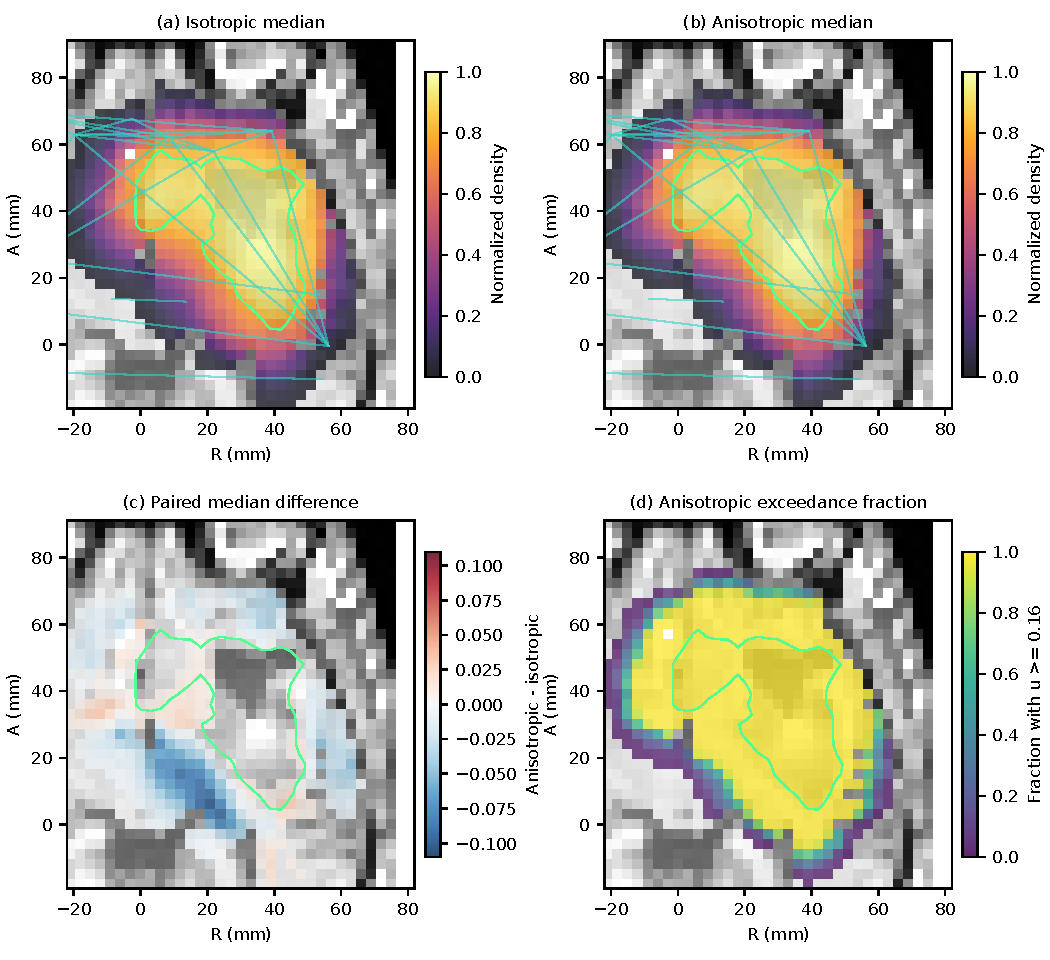
\includegraphics[width=\textwidth]{figures/pat16_fields.pdf}
\caption{PAT16 conditional day-90 growth on the preoperative axial plane at RAS $z=-12$ mm. (a,b) Pointwise marginal median normalized density with shared colors. (c) Median of paired anisotropic-minus-isotropic fields, with the full displayed difference range retained. (d) Fraction of assumed scenarios exceeding $u=0.16$, not a calibrated probability of tumor presence. Green contours show the input lesion at threshold 0.5. Cyan/purple lines in (a,b) are measured positive/negative FC projected from ROI centers within a $\pm12$ mm slab, not anatomical tracts on the slice. Background T1, lesion and FC are measurement-derived; growth is simulated. No functional decline is predicted. Values below 0.02 (absolute difference below 0.005 in panel c) are transparent for display only.}\label{fig:pat16_fields}
\end{figure}

The spatial comparison shows redistribution associated with directional transport (Figure~\ref{fig:pat16_fields}). Marginal global bands substantially overlapped throughout the run (Figure~\ref{fig:pat16_curves}). Regional mean-density summaries and measured static connectivity are supplied with the notebook; they do not constitute network or cognitive forecasts. No later patient scan was used to evaluate the hypothetical untreated evolution.

All paired initial states matched, and recorded densities remained between zero and 0.99733 without clipping. Every scenario used a 0.5-day step. For a representative central anisotropic scenario, halving the step changed day-90 density by \PATTimeDifference\% in relative $L^1$. A five-day pure-diffusion test gave relative mass error $5.69\times10^{-10}$ after float32 output storage. Additional tests verify tensor reconstruction and mixed derivatives, isotropic equivalence, a rotated Gaussian's covariance growth, coordinate transforms, conservation and blocked-corner behavior. These checks support implementation correctness and limited temporal sensitivity; spatial convergence on the PAT16 tissue graph and independent patient prediction have not been demonstrated.

\begin{figure}[tbp]
\centering
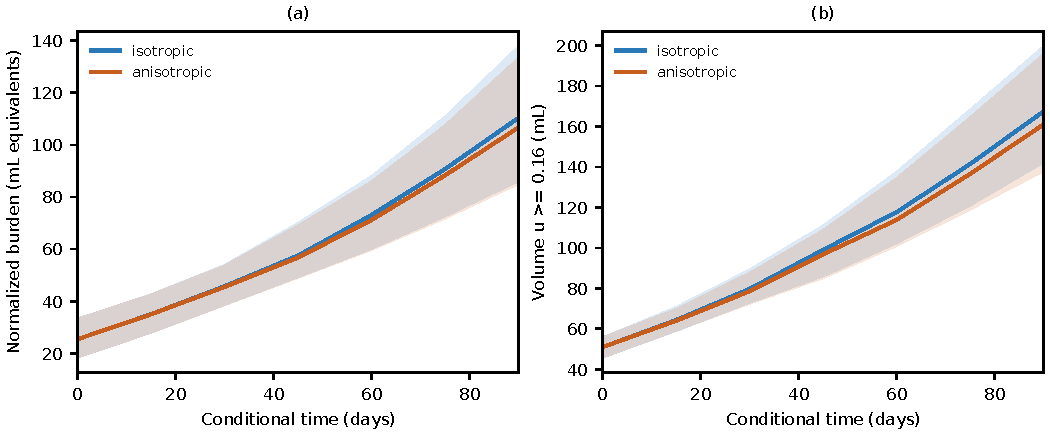
\includegraphics[width=\textwidth]{figures/pat16_timecourses.pdf}
\caption{PAT16 simulated normalized burden and illustrative threshold-defined volume. Lines are marginal medians and shading denotes 5th--95th empirical percentiles over the same \PATScenarios{} paired assumed scenarios. Time zero is lesion-based initialization, not tumor onset. No surgery, radiation, drug effect or oxygen limitation is included. Wide overlapping marginal bands coexist with the negative paired differences in Table~\ref{tab:pat16_outcomes}.}\label{fig:pat16_curves}
\end{figure}
\FloatBarrier
